\documentclass[12pt,a4paper]{report}
\usepackage[utf8]{inputenc}
\usepackage{amsmath}
\usepackage{amsfonts}
\usepackage{amssymb}
\usepackage{makeidx}
\usepackage{graphicx}
\usepackage{sectsty}
\usepackage{titlesec}
\usepackage{cite}
\usepackage{tikz}
\usepackage{tabularx}
\usepackage[left=4.00cm, right=3.00cm, top=3.00cm, bottom=3.00cm]{geometry}
\usetikzlibrary{shapes.geometric, arrows}
\usepackage[bahasa]{babel}
%===========================================
\renewcommand{\bibname}{Daftar Pustaka}
\renewcommand{\abstractname}{Abstraksi}
%===========================================
%CHAPTER FORMAT
\titleformat{\chapter}[display]{
	\LARGE \bfseries\centering
}{\chaptertitlename\ \thechapter}{5pt}{\large}
%CHAPTER SPACING
\titlespacing*{\chapter}{0pt}{30pt}{20pt}
%===========================================
\tikzstyle{startstop} = [rectangle, rounded corners, minimum width=3cm, minimum height=1cm,text centered, draw=black, fill=red!30]
\tikzstyle{io} = [trapezium, trapezium left angle=70, trapezium right angle=110, minimum width=3cm, minimum height=1cm, text centered, draw=black, fill=blue!30]
\tikzstyle{process} = [rectangle, minimum width=3cm, minimum height=1cm, text centered, draw=black, fill=orange!30]
\tikzstyle{decision} = [diamond, minimum width=3cm, minimum height=1cm, text centered, draw=black, fill=green!30]
\tikzstyle{arrow} = [thick,->,>=stealth]
%===========================================
%DOCUMENT START
\begin{document}
		\begingroup
		\thispagestyle{empty}  
		\begin{center}
			%TITLE
			\textbf{
				\Large
				Simulasi Sistem Penataan Wi-Fi dengan Algoritma Genetika\\[1cm]
				\normalsize
				Laporan Tugas Besar	
				\\[1cm]
				%AUTHOR
				Kelompok Keahlian : SIDE\\
				Kelompok 7\\[2cm]
				%LOGO
				
\includegraphics[width=0.35\linewidth]{logo}\\[2cm]
				%UNIVERSITY
				\Large
				Program Studi Sarjana Teknik Informatika\\
				Fakultas Informatika\\
				Universitas Telkom\\
				Bandung\\[0.2cm]
				2015}
		\end{center}
		\endgroup
		
		\tableofcontents
		\listoffigures
		\listoftables
		%=========================================
		\chapter*{Abstraksi}
			Saat ini penggunaan Wi-Fi (\emph{Wireless Fidelity}) untuk jaringan nirkabel sudah sangat umum. Namun, peletakan AP (\emph{Access Point}) terkadang kurang tepat. Sehingga, diperlukan optimasi penataan AP agar menghasilkan wilayah jangkauan yang optimal.
			
			Pada penelitian ini akan dilakukan pengukuran daya terima AP di Gedung B Fakultas Teknik Universitas Telkom dengan kriteria pengukuran level daya terima pada frekuensi kerja 2.4GHz. Selanjutnya akan dilakukan pemodelan sistem penataan Wi-Fi dengan algoritma genetika berdasarkan pada data hasil pengukuran untuk memperoleh wilayah jangkauan yang optimal.\\[0.5cm]
			\emph{\textbf{Kata kunci : } algoritma genetika, simulasi, wi-fi planner}
		\newpage
		%===========================================
		
		\chapter{Pendahuluan}
		\section{Latar Belakang}
		Penggunaan Wi-Fi pada jaringan lokal nirkabel sudah sangat umum. Kebutuhan untuk tetap terhubung pada jaringan lokal menuntut institusi untuk membangun infrastruktur jaringan lokal nirkabel yang optimal dari sisi jangkauan wilayah.
		
		Masalah yang sering ditemukan yaitu penataan Wi-Fi yang kurang memperhatikan jangkauan wilayah optimal. Penempatan Wi-Fi yang kurang optimal akan mengakibatkan bertambahnya jumlah AP yang dibutuhkan untuk menjangkau semua wilayah yang diinginkan yang pada akhirnya berdampak pada bertambahnya biaya. 
		
		Algoritma genetika digunakan sebagai algoritma untuk optimasi. Hasil akhir yang didapatkan yaitu nilai fitness yang maksimum berupa wilayah jangkauan optimal, mengacu pada data level daya terima dari AP. Kemudian akan dilakukan simulasi untuk penataan dengan keluaran nilai \emph{fitness} maksimum.
		\section{Perumusan Masalah}
		Dalam penelitian ini, permasalahan dirumuskan dalam bentuk pertanyaan sebagai berikut :
		\begin{enumerate}
			\item Bagaimanakah sistem penataan Wi-Fi yang baik agar mendapatkan wilayah jangkauan yang optimal di lingkungan nyata?
			\item Bagaimanakah menentukan sistem penataan Wi-Fi yang optimal dengan menggunakan algoritma genetika?
		\end{enumerate}
		\section{Tujuan}
		\begin{enumerate}
			\item Mengimplementasikan sistem penataan Wi-Fi yang optimal pada lingkungan nyata.
			\item Mengimplementasikan dan menganalisa penerapan algoritma genetika dalam menentukan sistem penataan Wi-Fi.
		\end{enumerate}
		\section{Batasan Masalah}
		Batasan masalah dalam simulasi ini adalah sebagai berikut :
		\begin{enumerate}
			\item Dengan banyaknya jenis perangkat AP, dalam penelitian ini digunakan TP-Link TL-WR741ND 802.11b/g/n dengan antena 5dBi Omni Directional.
			\item Lokasi penelitian terbatas pada Gedung B lantai dasar di Fakultas Teknik Universitas Telkom.
			\item Material bangunan dan cuaca tidak berpengaruh.
			\item Level daya terima diukur dengan menggunakan Kismet.
			\item Jika terdapat AP yang berdekatan, dipastikan bekerja pada kanal yang berbeda.
			\item Data letak AP yang ada di gedung B merupakan data masukan awal pada simulasi. Data ini berupa koordinat dalam sumbu X,Y berbeda.
			\item Solusi optimum dinilai dari daya jangkau tertinggi, terutama di titik kritis lokasi pengujian seperti square tengah, dan sepanjang koridor sekitar kelas.
		\end{enumerate}
		\section{Metodologi}
		Metodologi penyelesaian masalah yang dilakukan pada tugas besar ini adalah :
		\begin{enumerate}
			\item Studi Literatur
			
			Pada tahap ini dilakukan pengumpulan materi yang digunakan menjadi dasar teori untuk memperoleh deskripsi yang lebih jelas mengenai Wi-Fi, algoritma genetika, dan propagasi gelombang radio.
			
			\item Pengumpulan Data
			
			Pada tahap ini dilakukan pengumpulan data yang akan digunakan. Data berupa AP yang sudah ada di Gedung B Fakultas Teknik Universitas Telkom. Data tersebut kemudian direpresentasikan menjadi kromosom untuk  digunakan dalam algoritma genetika.
			
			\item Perancangan dan Implementasi
			
			Merancang dan membuat kakas yang mengimplementasikan metode algoritma genetika terhadap masalah yang dihadapi menggunakan bahasa python.
			
			\item Pengujian dan Analisis
			
			Pengujian sistem adalah dengan analisa wilayah jangkuan dari AP dan kemudian dilakukan simulasi dengan  algoritma genetika sehingga lokasi AP optimum.
			
			\item Penyusunan Laporan Tugas Besar
			
			Pada tahap ini dilakukan penyusunan laporan tertulis sebagai dokumentasi berdasarkan penelitian yang sudah dilakukan serta melampirkan kesimpulan dan saran dari hasil penelitian.
		\end{enumerate}
		
		
		\section{Jadwal Kegiatan}
		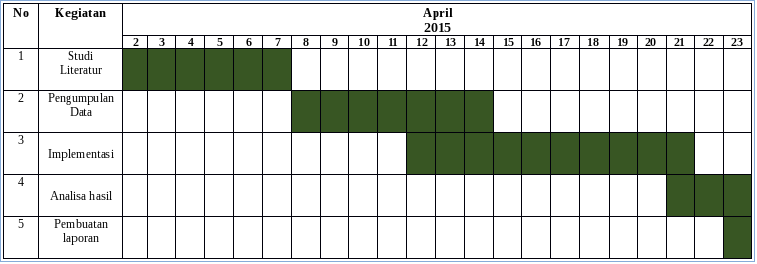
\includegraphics[width=\linewidth]{jadwal}
		\newpage
		%===========================================
		\chapter{Landasan Teori}
		\section{Gelombang Radio}
		Pada komunikasi nirkabel, digunakan media transmisi gelombang radio. Propagasi akan dilakukan untuk transmisi informasi. Propagasi gelombang radio adalah perambatan gelombang radio di suatu zat perantara. Propagasi gelombang radio dikatakan ideal jika gelombang yang dipancarkan pemancar diterima langsung tanpa hambatan oleh penerima.
		\subsection{\emph{Bandwidth}}
		\emph{Bandwith} adalah ukuran dari lebar daerah frekuensi. Jika lebar frekuensi yang digunakan oleh suatu perangkat adalah 2.40 GHz sampai 2.48 GHz maka \emph{bandwith} yang digunkan adalah 0.08 GHz. Semakin besar \emph{bandwith} yang digunakan akan berdampak pada semakin cepat atau besar jumlah data yang dapat dikirimkan didalamnya, dengan ilustrasi semakin lebar tempat yang tersedia di ruang frekuensi, semakin banyak data dapat kita masukkan pada sebuah waktu.\cite{Hartono2011}
		\subsection{Penyerapan Gelombang Radio}
		Pada saat gelombang elektromagnetik menabrak suatu material, biasanya gelombang akan menjadi lemah atau teredam \cite{Setiadi2013}. Banyak daya yang hilang akan sangat tergantung pada frekuensi yang digunakan dan tentunya material yang ditabrak. Untuk gelombang mikro, ada dua material utama yang menjadi penyerap \cite{Setiadi2013}, yaitu :
		\begin{enumerate}
			\item Logam
			
			Elektron bergerak bebas di metal dan siap untuk berayun oleh karenanya akan menyerap energy dari gelombang yang lewat.
			
			\item Air
			
			Gelombang mikro akan menyebabkan molekul air bergetar, yang pada prosesnya akan mengambil sebagian energi gelombang.
		\end{enumerate}
		Untuk kepentingan pembuatan jaringan nirkabel secara praktis, logam dan air akan dilihat sebagai penyerap gelombang yang baik. Lapisan air merupakan penghalang gelombang mikro. Air mempunyai banyak dampak yang besar. saat terjadi perubahan cuaca, sangat mungkin untuk membuat sambungan jaringan nirkabel menjadi putus \cite{Setiadi2013}.
		
		Ada material lain yang mempunyai efek yang lebih kompleks terhadap penyerapan gelombang radio, yaitu pohon atau kayu. Banyaknya penyerapan sangat tergantung pada jumlah air yang ada pada material yang terkena gelombang mikro \cite{Setiadi2013}.
		
		\section{\emph{Wireless Fidelity}}
		\emph{Wireless Fidelity} adalah standar untuk jaringan lokal nirkabel. Standar ini didasari oleh spesifikasi IEEE 802.11. Spesifikasi terbaru hingga saat ini yaitu 802.11ac. Secara berturut spesifikasi yang ada saat ini yaitu 802.11 b/g/n/ac.
		
		Versi Wi-Fi yang paling luas dalam pasaran saat ini beroperasi pada 2.400 MHz hingga 2.483,50 MHz. Pembagian operasi dalam 11 kanal yang berpusat di frekuensi berikut \cite{Kartika2010}:
		
		\begin{table}[h]
			\centering
			\begin{tabular}{|c|c|}
				\hline Kanal & Frekuensi \\ 
				\hline 1 & 2.412 \\ 
				\hline 2 & 2.417 \\ 
				\hline 3 & 2.422 \\ 
				\hline 4 & 2.427 \\ 
				\hline 5 & 2.432 \\ 
				\hline 6 & 2.437 \\ 
				\hline 7 & 2.442 \\ 
				\hline 8 & 2.447 \\ 
				\hline 9 & 2.452 \\ 
				\hline 10 & 2.457 \\ 
				\hline 11 & 2.462 \\ 
				\hline 
			\end{tabular} 
			\caption{Kanal Wi-Fi}
			\label{tab:kanal}
		\end{table}
		
		\section{Algoritma Genetika}
		AG (Algoritma genetika) adalah algoritma yang dikembangkan dari proses pencarian solusi optimasi secara acak. Populasi ini akan ber-evolusi menjadi populasi yang berbeda melalui serangkaian iterasi. Pada akhir iterasi, AG mengembalikan anggota populasi yang terbaik sebagai solusi untuk masalah tersebut. Pada setiap iterasi (generasi), proses evolusi yang terjadi adalah sebagai berikut:
		\begin{enumerate}
			\item Dua anggota populasi (induk) dipilih berdasarkan pada distribusi populasi. Induk kemudian dikawinkan melalui operator \emph{crossover} (pindah silang) untuk menghasilkan anak.
			
			\item Dengan probabilitas tertentu, anak ini akan mengalami perubahan oleh operator mutasi.
			
			\item Apabila anak sesuai untuk populasi tersebut, suatu skema penggantian diterapkan untuk memilih anggota populasi yang akan digantikan oleh anak.
			
			\item Proses ini terus berulang hingga dicapainya kondisi tertentu, misalnya hingga jumlah iterasi tertentu \cite{Suyanto2007}.
		\end{enumerate}
		
		\subsection{Reproduksi}
		Reproduski ini merupakan proses pergantian orang tua. Ada dua mekanisme yang digunakan untuk melakukan reproduski, yaitu cross over dan mutasi. Dengan adanya reproduksi ini memungkinkan bagi setiap individu dengan nilai \emph{fitness} terbaik untuk menjadi orang tua.
		\subsection{Pindah Silang}
		Pindah silang merupakan proses persilangan dua buah induk untuk mengahasilkan anak. Pada proses ini, titik potong pada kromosom bisa kromosom bisa dipilih lebih dari satu, semakin banyak titik potong yang dibuat, maka kualitas anak akan semakin menurun.
		\begin{figure}[h]
		\centering
		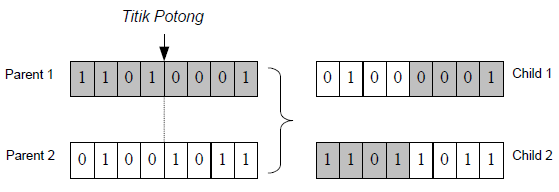
\includegraphics[width=0.7\linewidth]{crossover}
		\caption{\emph{Crossover} pada AG}
		\label{fig:crossover}
		\end{figure}

		\subsection{Mutasi}
		Mutasi merupakan proses pergantian gen dalam kromosom anak yang hilang akibat adanya pindah silang. Kejadian mutasi ini umumnya memiliki probabilitas kecil, jika dilakukan terlalu sering, maka akan menghasilkan individu yang lemah \cite{Suyanto2007}.
		\begin{figure}[h]
			\centering
			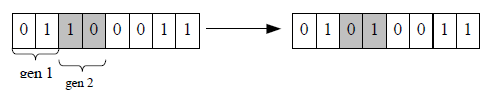
\includegraphics[width=0.7\linewidth]{mutasi}
			\caption{Mutasi pada AG}
			\label{fig:mutasi}
		\end{figure}
		
		\subsection{\emph{Roulette Wheel}}
		\emph{Roulette Wheel} ini digunakan untuk melakukan pemilihan orang tua. Pembuatan \emph{Roulette Wheel} ini berdasarkan nilai \emph{fitness} tiap kromosom yang akan dipilih menjadi orang tua. Individu yang memiliki nilai \emph{fitness} tertinggi memiliki peluang untuk terpilih.
		\begin{figure}[h]
		\centering
		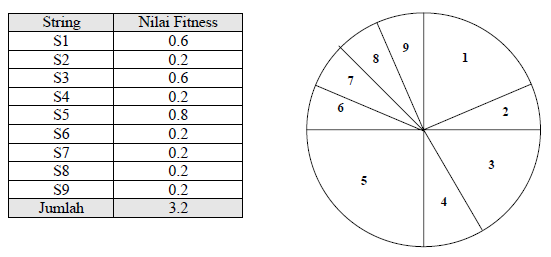
\includegraphics[width=0.7\linewidth]{roulette}
		\caption{Roulette Wheel pada AG}
		\label{fig:roulette}
		\end{figure}


		\subsection{Pergantian Individu}
		Ada dua mekanisme yang bisa dipilih untuk melakukan pergantian individu, yaitu : 
		\begin{enumerate}
			\item Mengganti orang tua dengan nilai \emph{fitness} terkecil.
			
			\item Membandingkan anak dengan orang tua, jika anak memiliki nilai fitness lebih baik dibandingkan dengan orang tua, maka anak akan menggantikan orang tua dalam populasi \cite{Suyanto2007}.
		\end{enumerate}
		
		
		\subsection{Penghentian}
		Ada dua mekanisme penghentian yang bisa dipilih, yaitu :	
		\begin{enumerate}
			\item Menentukan sebuah nilai sebagai batas iterasi.
			
			\item Menghitung kegagalan penggantian anggota populasi secara berturut-turut sampai jumlah tertentu.
		\end{enumerate}
		\newpage
		
		%==========================================================
		\chapter{Perancangan Sistem}
		\section{Gambaran Umum Sistem}
		Pemodelan sistem dilakukan dengan posisi access point di lokasi sebenarnya. Lokasi pengambilan data akan digambarkan dalam bentuk citra tiga dimensi yang dimulai dari koordinat (0,0,0). Dengan arah pertambahan sumbu X ke kanan, arah pertambahan sumbu Y ke bawah, dan arah penambahan sumbu Z ke atas. Setelah itu, wilayah jangkauan akan divisualisasikan dengan warna hijau untuk wilayah yang mampu dijangkau, dan merah untuk yang tidak terjangkau. Kemudian, akan dilakukan pemodelan dengan AG untuk optimasi wilayah jangkauan AP. Inisialisasi populasi mengacu pada posisi AP sebenarnya. Kemudian akan dicari nilai \emph{fitness} berdasarkan pada wilayah jangkauan yang terbesar.
		\subsection{Deskripsi Tahapan Proses}
		\begin{center}
			\begin{tikzpicture}[node distance=2.5cm]
			\node (start) [startstop] {Mulai};
			\node (in1) [io, below of=start] {Data Lokasi AP};
			\node (pro1) [process, below of=in1] {Membangun Solusi dengan AG};
			\node (pro2) [process, below of=pro1] {Analisis Solusi};
			\node (dec1) [decision, below of=pro2] {optimum?};
			\node (out1) [io, below of=dec1] {Solusi Akhir};
			\node (end) [startstop, below of=out1] {Selesai};
			
			\draw [arrow] (start) -- (in1);
			\draw [arrow] (in1) -- (pro1);
			\draw [arrow] (pro1) -- (pro2);
			\draw [arrow] (pro2) -- (dec1);
			\draw [arrow] (dec1)-| node{tidak} ([xshift=1cm]pro1.south east) |- (pro1);
			\draw [arrow] (dec1) -- node{ya} (out1);
			\draw [arrow] (out1) -- (end);
			\end{tikzpicture}
		\end{center}
		\subsection{Data Lokasi AP}
		Data awal diambil dari lokasi AP yang ada di gedung B. Sesuai penjelasan sebelumnya bahwa data berupa koordinat AP pada sumbu (X,Y). Sehingga, digambarkan bidang dengan titik (0,0) merupakan lokasi jalan masuk dari gedung B lantai satu, dengan sumbu X positif merupakan arah timur dan sumbu Y positif merupakan arah utara.
		
		Dari hasil observasi, diperoleh bahwa jumlah AP di gedung B lantai dasar berjumlah sebelas buah. Sehingga dihasilkan data awal sebagai berikut.
		\subsection{Membentuk Solusi dengan Algoritma Genetika}
		Pada tahap ini dilakukan pencarian solusi dengan menggunakan AG. Solusi dikatakan optimum jika wilayah  gedung B mampu dijangkau oleh AP. AG melakukan beberapa tahapan proses dalam mencari solusi, yaitu :
		\begin{enumerate}
			\item Inisialisasi populasi
			\item Evaluasi individu
			\item Seleksi orangtua
			\item Perkawinan
			\item Mutasi
		\end{enumerate}
		\subsubsection{Inisialisasi Populasi}
		Inisialisai populasi dilakukan dengan membuat 15 individu. Tiap individu merupakan kerangka gedung B dalam bentuk diagram kartesius dengan sebelas lokasi AP yang terletak secara acak dalam koordinat x,y. Kerangka gedung B ini terdiri dari 80x30 kotak, dimana tiap kotak mewakili satu $ m^{2} $ pada gedung B yang sebenarnya. Tiap kotak ini terletak pada koordinat $x,y$ dan menjadi lokasi penempatan AP di simulasi.
		\subsubsection{Evaluasi Individu}
		Evaluasi individu atau sering disebut nilai \emph{fitness} merupakan nilai kesesuaian individu untuk menjadi solusi. Ada berbagai cara untuk menentukan nilai \emph{fitness} dari individu. Pada simulasi ini, nilai \emph{fitness} sebuah individu dihitung dengan cara banyaknya kotak yang ter-\emph{cover} oleh AP. Semakin banyak kotak yang ter-\emph{cover} oleh AP, maka nilai \emph{fitness} individu tersebut semakin tinggi. Tiap AP mempunyai \emph{coverage area} dengan diameter 12 kotak. Jadi secara matematis, rumus nilai \emph{fitness} dapat dihitung dengan
		\[ fitness=\frac{\sum kotak tercover}{\sum total kotak} \]
		
		\subsubsection{Seleksi Orangtua}
		Seleksi orang tua dilakukan dengan menggunakan \emph{Roulette Wheel}. Setelah diperoleh nilai \emph{fitness} tiap individu dalam populasi, kemudian tiap individu ditempatkan dalam sebuah lingkaran dengan proporsi sesuai dengan nilai fitness. Setelah itu di-\emph{generate} sebuah nilai dengan distribusi normal. Nilai yang keluar kemudian digunakan untuk memilih individu sesuai dengan nilai \emph{fitness} yang ada di \emph{Roulette Wheel}.
		\subsubsection{Perkawinan}
		Setelah didapat dua orang tua, kemudian dilakukan perkawinan dengan melakukan \emph{crossover}. Penentuan lokasi titik potong \emph{crossover} merupakan acak dan perpotongan yang dilakukan berdasarkan kolom. Setelah dipotong, kemudian bagian yang terpotong dari dua orang tua dipertukarkan.
		\subsubsection{Mutasi}
		Setiap anak hasil persilangan memiliki probabilitas mutasi, jika probabilitasnya sesuai, maka anak tersebut akan mengalami mutasi. Mutasi dilakukan dengan merubah lokasi AP dari satu kotak ke kotak lain. 
		
		\subsection{Analisis Solusi}
		Analisis dilakukan dengan menggunakan perangkat lunak Kismet. Perangkat ini digunakan untuk mengukur level daya terima sinyal Wi-Fi sebuah \emph{device}. Pengujian akan dilakukan pada lokasi terjauh pada gedung B dari lokasi AP. 
		
		\subsection{Solusi Akhir}
		Solusi akhir yang masih dalam bentuk kromosom hasil dari sistem kemudian diubah menjadi koordinat sehingga bisa diimplementasikan.
		
		\newpage
		%==========================================================
		\chapter{Pengujian dan Analisis}
		\section{Pengujian}
		Pengujian dilakukan pada matriks berukuran 80 x 30 dengan representasi nilai 0 sebagai wilayah tidak ter-\emph{cover} dan nilai 1 sebagai wilayah ter-\emph{cover}.
		
		Dari hasil simulasi terhadap data yang ada. Dilakukan pengujian dengan AG, kemudian dihasilkan nilai \emph{fitness} sebagai berikut :

		\begin{table}[h]
			\centering
			\begin{tabular}{|c|c|}
				\hline \textbf{\emph{Test Case}} & \textbf{\emph{Fitness}} \\ 
				\hline 1 & 0.93 \\ 
				\hline 2 & 0.98 \\ 
				\hline 3 & 0.92 \\ 
				\hline 4 & 0.91 \\ 
				\hline 5 & 0.90 \\ 
				\hline 6 & 0.92 \\ 
				\hline 7 & 0.96 \\ 
				\hline 8 & 0.95 \\ 
				\hline 9 & 0.93 \\ 
				\hline 10 & 0.93 \\ 
				\hline 
			\end{tabular}
			\caption{Data hasil pengujian dengan AG}
			\label{tab:1}
		\end{table}
		Data pada Tabel \ref{tab:1} akan digunakan sebagai bahan untuk analisis hasil.
		\section{Analisis}
		Berdasarkan pada data dari hasil pengujian, nilai \emph{fitness} tertinggi terdapat pada nilai 0.98 (maksimal 1) yang terdapat pada generasi ke-0 \emph{test case} kedua, dengan detail koordinat lokasi AP yaitu [5, 63], [7, 77], [9, 21], [9, 45], [11, 5], [15, 64], [17, 48], [25, 6], [25, 28], [26, 73], dan [28, 61]. Adapun hasil visualisasi dari individu tersebut seperti pada Gambar \ref{fig:apLoc_02} dan Gambar \ref{fig:coverage_02}.
		
		Namun, jika dilihat dari titik-titik kritis pada Gedung B, individu yang paling optimal yaitu pada individu dengan koordinat [1, 54], [2, 9], [2, 14], [17, 41], [10, 27], [11, 3], [12, 71], [13, 41], [13, 12], [23, 52], dan [28, 13] seperti pada Gambar \ref{fig:apLoc_05}, dengan visualisasi \emph{coverage area} seperti pada Gambar \ref{fig:coverage_05}
		
		\begin{figure}[h]
			\centering
			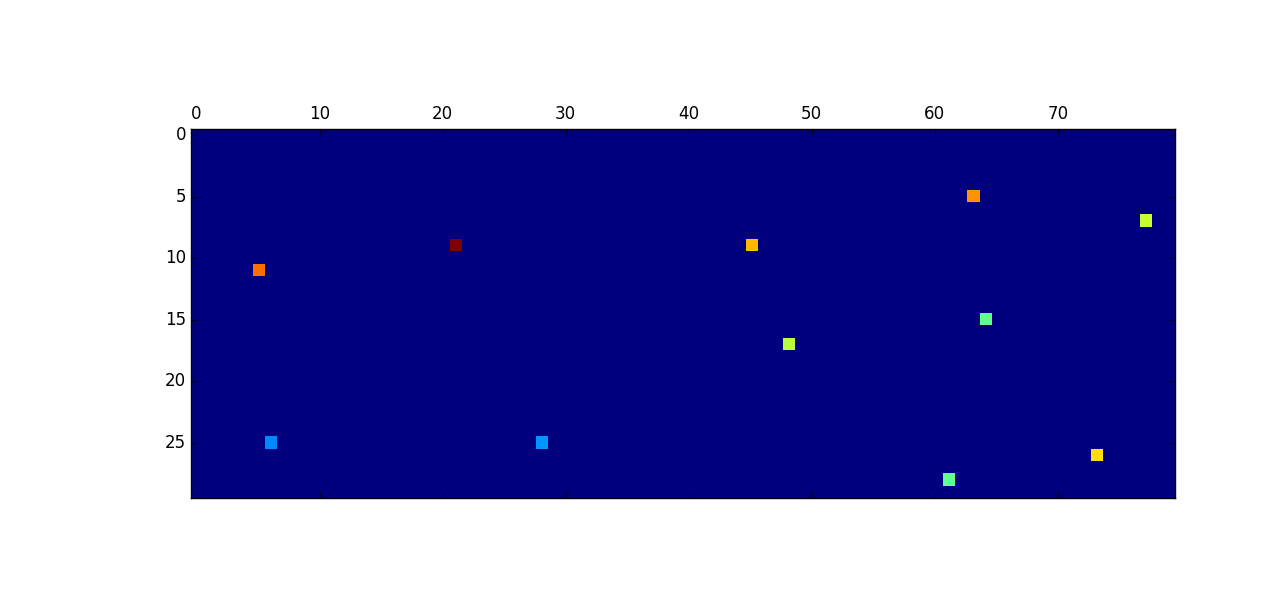
\includegraphics[width=0.5\linewidth]{apLoc_02}
			\caption{Koordinat lokasi AP individu A}
			\label{fig:apLoc_02}
		\end{figure}	
		
		\begin{figure}[h]
			\centering
			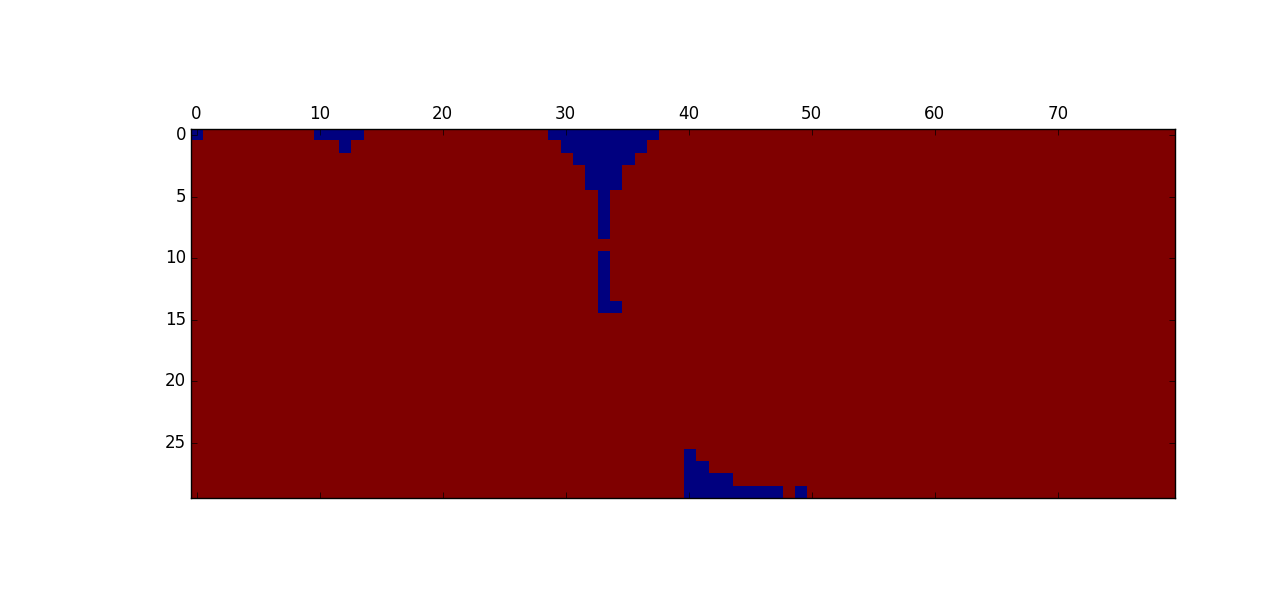
\includegraphics[width=0.5\linewidth]{coverage_02}
			\caption{\emph{coverage area} individu A}
			\label{fig:coverage_02}
		\end{figure}
		
		\begin{figure}[h]
		\centering
		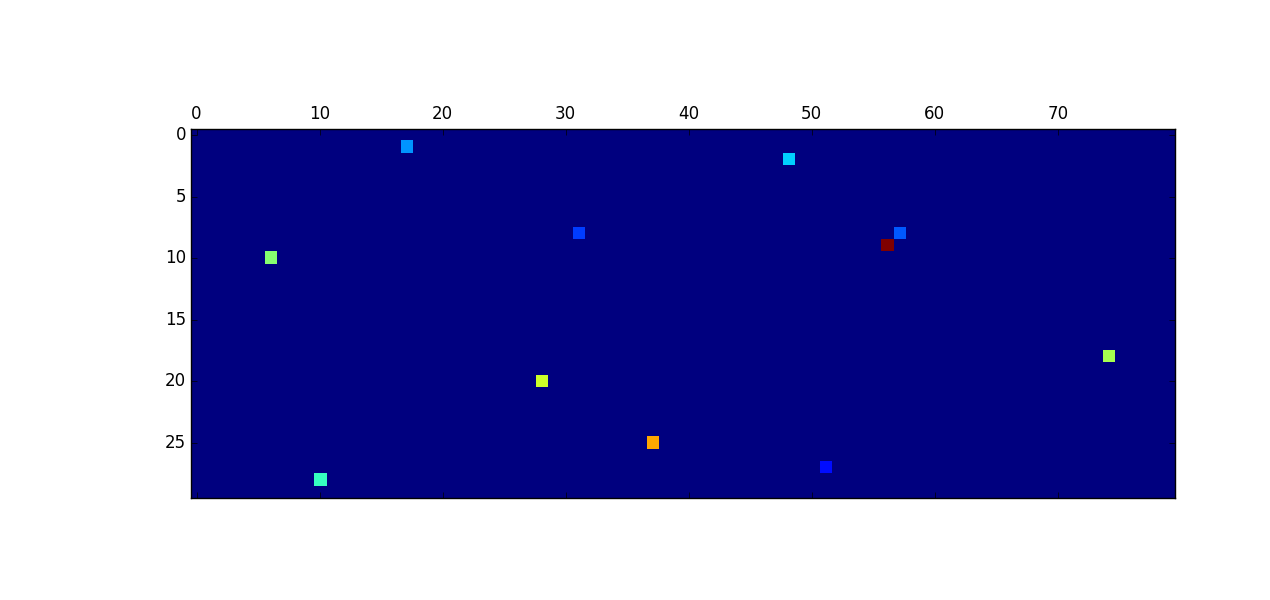
\includegraphics[width=0.5\linewidth]{apLoc_05}
		\caption{Koordinat lokasi AP individu B}
		\label{fig:apLoc_05}
		\end{figure}
		
		\begin{figure}[h]
		\centering
		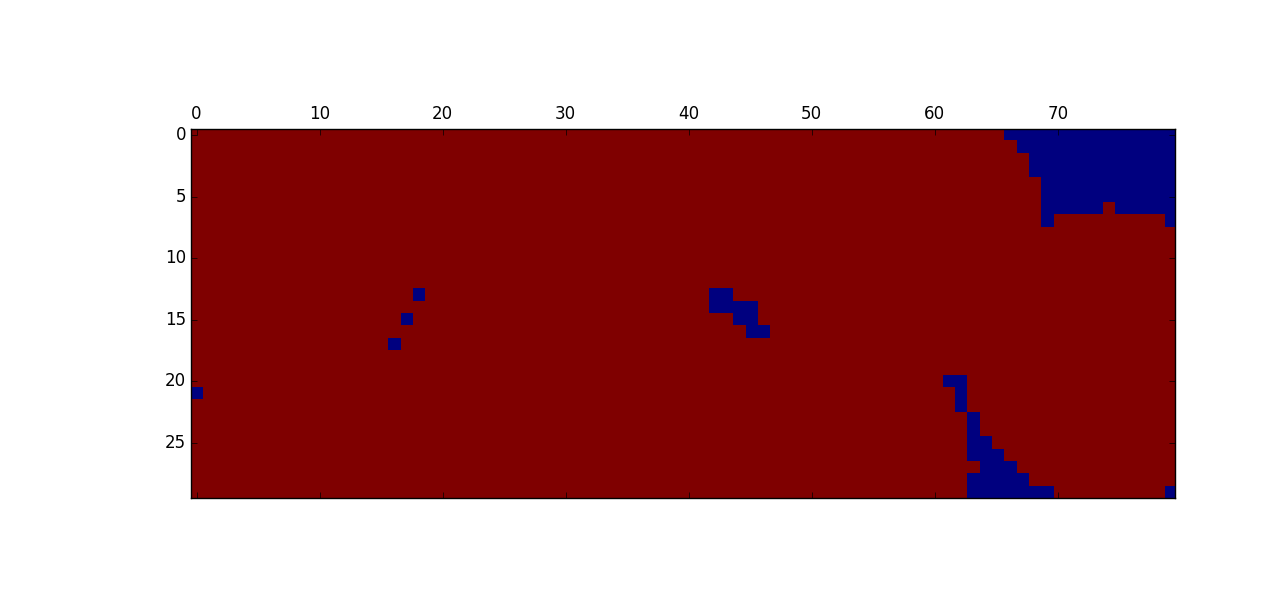
\includegraphics[width=0.5\linewidth]{coverage_05}
		\caption{\emph{coverage area} individu B}
		\label{fig:coverage_05}
		\end{figure}
		
		Jika dilakukan perbandingan, individu A lebih unggul jika mengacu terhadap nilai \emph{fitness}. Namun, individu B lebih unggul jika mengacu terhadap aplikasi di lingkungan nyata. Karena, pada individu A terdapat \emph{blank spot} tepat di titik krisis Gedung B (bagian tengah).
		%==========================================================
		\chapter{Kesimpulan dan Saran}
		\section{Kesimpulan}
		Berdasarkan pada hasil pengujian dan analisis, terdapat beberapa kesimpulan dari penelitian ini yaitu:
		\begin{itemize}
			\item Individu A paling optimal jika ditinjau dari nilai \emph{fitness} yang dimiliki.
			\item Individu B paling optimal jika ditinjau dari aplikasinya di lingkungan nyata. Karena, pada individu B titik kritis di Gedung B masih cukup tertutupi, sementara di bagian sisi ujung (toilet) tidak ter-\emph{cover}.
			\item Individu A kurang cocok diimplementasikan pada lingkungan nyata karena terdapat \emph{blank spot} pada titik krisis di Gedung B, yaitu bagian tengah yang notabenenya ramai pengguna.
		\end{itemize}
		\section{Saran}
		Dari hasil penelitian ini, perlu kajian lebih lanjut untuk mendapatkan hasil yang lebih optimal. Pada penelitian selanjutnya dapat dikaji kembali dengan memperhitungkan parameter lain seperti pengaruh material dan cuaca terhadap daya pancar AP. Selain itu, diperlukan kajian lebih lanjut dalam proses implementasi AG seperti pada metode \emph{crossover} yang baik, fungsi acak untuk peletakan AP berdasar pada AP sebelumnya.
		%=========================================
		\bibliographystyle{ieeetr}
		\bibliography{laporanreferensi}
\end{document}